\documentclass{standalone}
\usepackage{graphicx}	
\usepackage{amssymb, amsmath, amsthm}
\usepackage{color}

\usepackage{tikz}
\usetikzlibrary{intersections, backgrounds, math}

\definecolor{light}{RGB}{220, 188, 188}
\definecolor{mid}{RGB}{185, 124, 124}
\definecolor{dark}{RGB}{143, 39, 39}
\definecolor{highlight}{RGB}{180, 31, 180}
\definecolor{darkteal}{RGB}{29, 79, 79}
\definecolor{darkolive}{RGB}{97, 123, 45}
\definecolor{gray10}{gray}{0.1}
\definecolor{gray20}{gray}{0.2}
\definecolor{gray30}{gray}{0.3}
\definecolor{gray40}{gray}{0.4}
\definecolor{gray60}{gray}{0.6}
\definecolor{gray70}{gray}{0.7}
\definecolor{gray80}{gray}{0.8}
\definecolor{gray90}{gray}{0.9}
\definecolor{gray95}{gray}{0.95}

\begin{document}

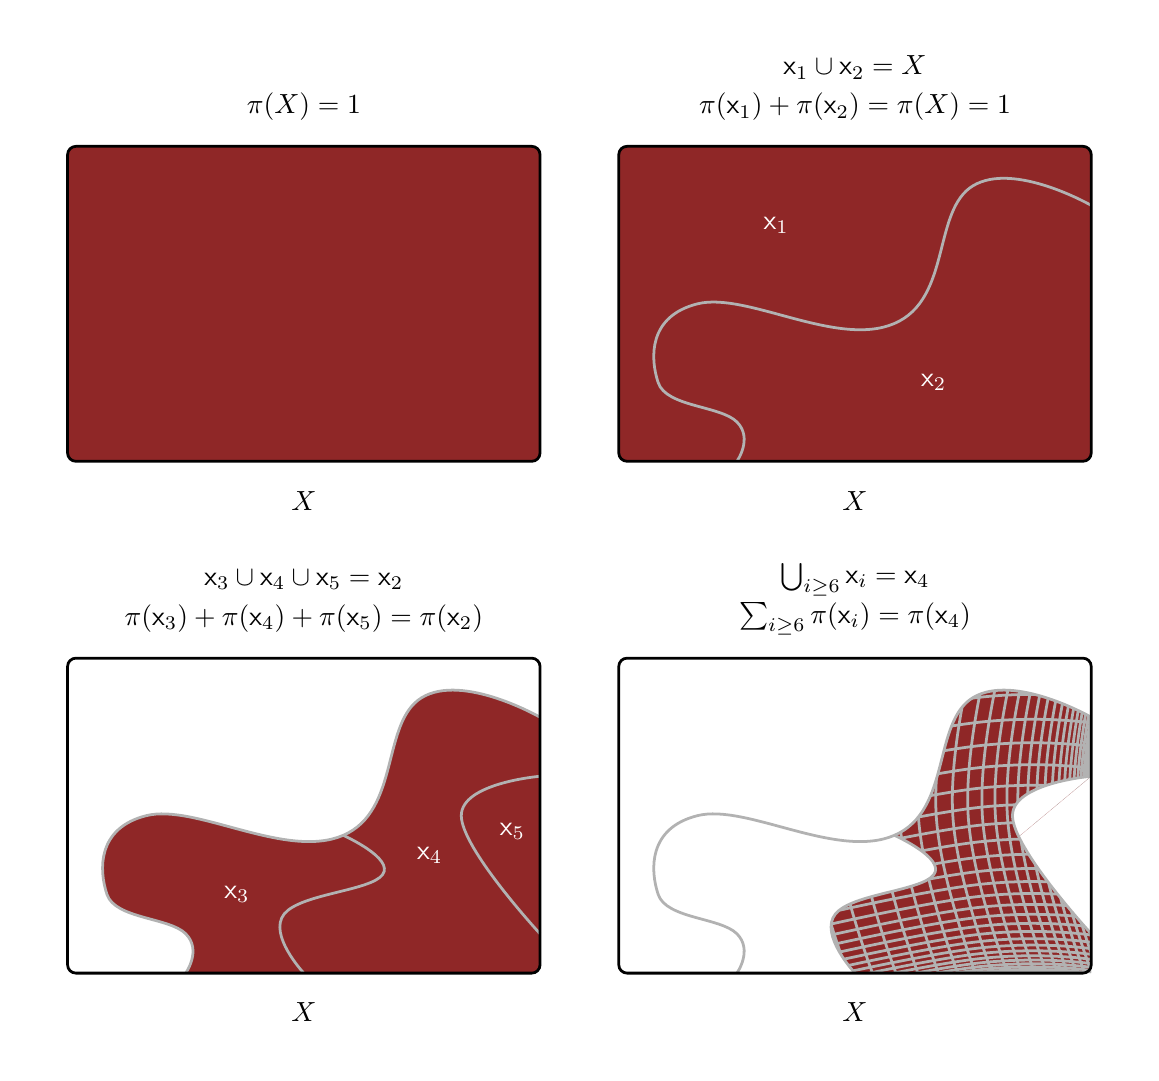
\begin{tikzpicture}[scale=1.0]
  
  \begin{scope}[shift={(0, 0)}]
    \draw[white] (-3.5, -3) rectangle (3.5, 3.5);
  
    \fill[rounded corners=3, dark] (-3, -2) rectangle (3, 2);
  
    \draw[rounded corners=3, black, line width=1] (-3, -2) rectangle (3, 2);
    \node at (0, -2.5) { $X$ };
    
    \node at (0, 2.5) { $\pi(X) = 1$ };
  \end{scope}
  
  \begin{scope}[shift={(7, 0)}]
    \draw[white] (-3.5, -3) rectangle (3.5, 3.5);
      
    \fill[rounded corners=3, dark] (-3, -2) rectangle (3, 2);
      
    \draw[gray70, line width=1] plot [smooth, tension=0.75] coordinates { 
      (-1.5, -2) (-1.5, -1.5) (-2.5, -1) (-2, 0) (0.5, -0.25) (1.5, 1.5) (3, 1.25) };
      
    \node[white] at (-1, 1) { $\mathsf{x}_{1}$ };
    \node[white] at (1, -1) { $\mathsf{x}_{2}$ };
      
    \draw[rounded corners=3, color=black, line width=1] (-3, -2) rectangle (3, 2);
    \node at (0, -2.5) { $X$ };
    
    \node at (0, 3) { $\mathsf{x}_{1} \cup \mathsf{x}_{2} = X$ };
    \node at (0, 2.5) { $\pi(\mathsf{x}_{1}) + \pi(\mathsf{x}_{2}) = \pi(X) = 1$ };
  \end{scope}

  \begin{scope}[shift={(0, -6.5)}]
    \draw[white] (-3.5, -3) rectangle (3.5, 3.5);
      
    \begin{scope}
      \clip[rounded corners=3] (-3, -2) rectangle (3, 2);
      \fill[dark, line width=1] plot [smooth, tension=0.75] coordinates { 
        (-1.5, -2) (-1.5, -1.5) (-2.5, -1) (-2, 0) (0.5, -0.25) (1.5, 1.5) (3, 1.25) }
        -- (3, -2) -- (-1.5, -2);
    \end{scope}
    
    \draw[gray70, line width=1] plot [smooth, tension=0.75] coordinates { 
      (-1.5, -2) (-1.5, -1.5) (-2.5, -1) (-2, 0) (0.5, -0.25) (1.5, 1.5) (3, 1.25) };
      
    \draw[gray70, line width=1] plot [smooth, tension=0.75] coordinates { 
      (0, -2) (-0.25, -1.25) (1, -0.75) (0.5, -0.25)  };
    
    \draw[gray70, line width=1] plot [smooth, tension=0.75] coordinates { 
      (3, 0.5) (2, 0) (3, -1.5)  };
      
    \node[white] at (-0.85, -1) { $\mathsf{x}_{3}$ };
    \node[white] at (1.6, -0.5) { $\mathsf{x}_{4}$ };
    \node[white] at (2.65, -0.2) { $\mathsf{x}_{5}$ };
    
    \draw[rounded corners=3, color=black, line width=1] (-3, -2) rectangle (3, 2);
    \node at (0, -2.5) { $X$ };
    
    \node at (0, 3) { $\mathsf{x}_{3} \cup \mathsf{x}_{4} \cup \mathsf{x}_{5} = \mathsf{x}_{2}$ };
    \node at (0, 2.5) { $\pi(\mathsf{x}_{3}) + \pi(\mathsf{x}_{4}) + \pi(\mathsf{x}_{5}) = \pi(\mathsf{x}_{2}) $ };
  \end{scope}
  
  \begin{scope}[shift={(7, -6.5)}]
    \draw[white] (-3.5, -3) rectangle (3.5, 3.5);
    
    \begin{scope}
      \clip plot [smooth, tension=0.75] coordinates { 
        (-1.5, -2) (-1.5, -1.5) (-2.5, -1) (-2, 0) (0.5, -0.25) (1.5, 1.5) (3, 1.25) }
        -- (3, -2) -- (-1.5, -2);
       
      \begin{scope}
        \clip plot [smooth, tension=0.75] coordinates { (0, -2) (-0.25, -1.25) (1, -0.75) (0.5, -0.25)  }
        -- (0.5, 2) -- (3, 2) -- (3, 0.5)
        plot [smooth, tension=0.75] coordinates { (3, 0.5) (2, 0) (3, -1.5)  }
        -- (3, -2) -- (0, -2);
        
        \fill[rounded corners=3, dark] (-3, -2) rectangle (3, 2);
        
        \foreach \n in {1, 2, ..., 50} {
          \pgfmathsetmacro{\y}{-2.1 + 0.1 * exp(3 * ln(0.1 * \n))}
          \draw[gray70, line width=1] plot [smooth, tension=0.75] coordinates { 
            (-1, \y - 0.5) (1.5, \y) (3, \y) };
        }
    
        \foreach \n in {1, 2, ..., 50} {
          \pgfmathsetmacro{\x}{3.5 - 0.1 * exp(3 * ln(0.1 * \n))}
          \draw[gray70, line width=1] plot [smooth, tension=0.75] coordinates { 
             (\x, -2) (\x - 0.5, 0) (\x - 0.25, 2) };
        }
      \end{scope}
    \end{scope}
    
    \draw[gray70, line width=1] plot [smooth, tension=0.75] coordinates { 
      (-1.5, -2) (-1.5, -1.5) (-2.5, -1) (-2, 0) (0.5, -0.25) (1.5, 1.5) (3, 1.25) };
      
    \draw[gray70, line width=1] plot [smooth, tension=0.75] coordinates { 
      (0, -2) (-0.25, -1.25) (1, -0.75) (0.5, -0.25)  };
    
    \draw[gray70, line width=1] plot [smooth, tension=0.75] coordinates { 
      (3, 0.5) (2, 0) (3, -1.5)  };
    
    \draw[rounded corners=3, color=black, line width=1] (-3, -2) rectangle (3, 2);
    \node at (0, -2.5) { $X$ };
    
    \node at (0, 3) { $\bigcup_{i \ge 6} \mathsf{x}_{i} = \mathsf{x}_{4}$ };
    \node at (0, 2.5) { $\sum_{i \ge 6} \pi(\mathsf{x}_{i}) = \pi(\mathsf{x}_{4}) $ };
    
  \end{scope}
  
\end{tikzpicture}

\end{document}  